\section{固定分布下的直接求导}
\label{sec:pgrad-direct}

最简单的情形是图~\ref{fig:pgrad-three-entries}(a)：抽样分布$P$与参数无关，参数只出现在函数里，$J(\bm{\theta})=\mathbb{E}_{P}[f_{\bm{\theta}}(X)]$。这时可以先在每个样本处对函数求导，再取平均吗？

\paragraph{梯度表示}

在定理~\ref{thm:pgrad-exchange}中取$\mu=P$、$g(\bm{\theta},x)=f_{\bm{\theta}}(x)$。若$f_{\bm{\theta}_{0}}$在$P$下可积，对$P$几乎所有$x$在$\bm{\theta}_{0}$处可微，并且在$\bm{\theta}_{0}$的某个开球$U$上满足式~\eqref{eq:pgrad-lipschitz}的可积控制，则
\begin{equation}
  \nabla J(\bm{\theta})=\mathbb{E}_{P}\bigl[\nabla_{\bm{\theta}}f_{\bm{\theta}}(X)\bigr].
  \label{eq:pgrad-direct}
\end{equation}
梯度本身成了一个期望，被积函数是逐样本的导数$\bm{G}=\nabla_{\bm{\theta}}f_{\bm{\theta}}(X)$。卷五的随机梯度方法就是在这种情形下使用样本梯度的，相应的交换引理可参考\BookChapterRef{chap:stochastic-gradient-methods}{卷五第13章“随机梯度方法”}。

\paragraph{样本估计}

取$X_{1},\dots,X_{n}$独立同分布于$P$，令
\begin{equation}
  \hat{\bm{g}}_{n}^{\mathrm{dir}}=\frac{1}{n}\sum_{i=1}^{n}\nabla_{\bm{\theta}}f_{\bm{\theta}}(X_{i}).
  \label{eq:pgrad-direct-estimator}
\end{equation}
这就是第~\ref{chap:monte-carlo-integration-error}章的样本平均，只不过被平均的是一个$\mathbb{R}^{k}$值函数。对它要问两件事，所需的条件不同。

第一件是期望与一致性。定理~\ref{thm:pgrad-exchange}的证明已经给出$\lVert\bm{G}\rVert_{2}\leq\sqrt{k}M(X)$，所以$\bm{G}$可积。由期望的线性，$\hat{\bm{g}}_{n}^{\mathrm{dir}}$的期望就是$\nabla J(\bm{\theta})$，估计无偏；对每个分量用强大数律（第~\ref{chap:laws-of-large-numbers}章），$\hat{\bm{g}}_{n}^{\mathrm{dir}}$几乎必然收敛到$\nabla J(\bm{\theta})$。这两条只用到一阶矩。

第二件是误差的大小。若$\mathbb{E}\lVert\bm{G}\rVert_{2}^{2}<\infty$，记$\bm{G}$的协方差矩阵为$\bm{\Sigma}_{\bm{G}}$，则各分量独立同分布平均的方差是$(\bm{\Sigma}_{\bm{G}})_{j,j}/n$，相加得到均方误差
\begin{equation}
  \mathbb{E}\bigl\lVert\hat{\bm{g}}_{n}^{\mathrm{dir}}-\nabla J(\bm{\theta})\bigr\rVert_{2}^{2}=\frac{\operatorname{tr}\bm{\Sigma}_{\bm{G}}}{n}.
  \label{eq:pgrad-direct-mse}
\end{equation}
这是熟悉的$n^{-1/2}$误差尺度。没有二阶矩时上式右边是无穷，大数律仍然成立，但误差缩小的速度可以慢得多。导数的可积性支撑“算得对”，导数的平方可积性才支撑“算得多准”。

\paragraph{一个只有一阶矩的例子}

设$X$的密度为$3x^{-4}$（$x\geq1$），$f_{\theta}(x)=x^{\theta}$。对$\theta<3$，
\[
  J(\theta)=\int_{1}^{\infty}x^{\theta}\cdot3x^{-4}\,\mathrm{d}x=\frac{3}{3-\theta},
\]
$\theta\geq3$时积分发散，所以只在$\theta<3$上讨论。逐样本导数是$G=X^{\theta}\ln X$。

先检查交换条件。取$\delta>0$使$\theta+\delta<3$，在$U=(\theta-\delta,\theta+\delta)$上
\[
  \bigl\lvert\partial_{\theta'}x^{\theta'}\bigr\rvert=x^{\theta'}\ln x\leq x^{\theta+\delta}\ln x,\qquad x\geq1,
\]
右边在$X$的分布下可积，因为
\[
  \int_{1}^{\infty}x^{\theta+\delta}\ln x\cdot3x^{-4}\,\mathrm{d}x=\frac{3}{(3-\theta-\delta)^{2}}<\infty .
\]于是由式~\eqref{eq:pgrad-direct}，
\[
  J'(\theta)=\mathbb{E}[X^{\theta}\ln X]=\frac{3}{(3-\theta)^{2}},
\]
与直接对$3/(3-\theta)$求导一致。

再看二阶矩。分部积分两次可得，对$a>1$，
\[
  \int_{1}^{\infty}x^{-a}\ln^{2}x\,\mathrm{d}x=\frac{2}{(a-1)^{3}} .
\]
取$a=4-2\theta$，得到
\[
  \mathbb{E}[G^{2}]=3\int_{1}^{\infty}x^{2\theta-4}\ln^{2}x\,\mathrm{d}x=\frac{6}{(3-2\theta)^{3}},\qquad\theta<\tfrac{3}{2},
\]
$\theta\geq\frac{3}{2}$时为无穷。在$\theta=1$处$J'(1)=\frac{3}{4}$，$\mathbb{E}[G^{2}]=6$，单样本方差$6-\frac{9}{16}=\frac{87}{16}\approx5.44$。在$\theta=2$处$J'(2)=3$，导数可积而方差无穷。

手算时用逆变换采样（第~\ref{chap:sample-generation}章）：分布函数是$1-x^{-3}$，于是$X=(1-U)^{-1/3}$。取均匀数$u=0.37,0.80,0.15,0.62$，得
\[
  X=1.1665,\ 1.7100,\ 1.0557,\ 1.3806 .
\]
在$\theta=1$处，四个导数样本$G=X\ln X$是
\[
  G=0.1797,\ 0.9174,\ 0.0572,\ 0.4453,
\]
平均为$0.3999$，真值是$0.75$。偏离约$0.35$，而四样本平均的标准差是$\sqrt{5.44/4}\approx1.17$，这个偏离在正常波动范围内。

图~\ref{fig:pgrad-pareto-paths}把样本数加到两万。$\theta=1$时各条路径在几百个样本后就贴近真值；$\theta=2$时路径长时间偏低，偶尔被一个巨大的样本拉高，然后再缓慢回落。这是无穷方差下的典型样子：绝大多数样本偏小，期望里相当一部分来自稀少的大值。

\begin{BookInlineFigure}
  \centering
  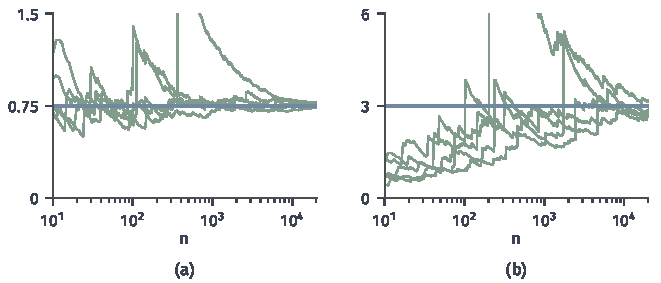
\includegraphics[width=112mm]{figures/07-probability/08-sampling-and-integration/matplotlib/pgrad-pareto-paths/figure.pdf}
  \caption{密度为$3x^{-4}$（$x\geq1$）时，导数样本$X^{\theta}\ln X$的运行平均，横轴为样本数$n$（对数刻度）。绿线为五条固定种子的独立路径，蓝线为真值$J'(\theta)=3/(3-\theta)^{2}$。(a)$\theta=1$，导数有有限方差；(b)$\theta=2$，导数可积但方差无穷。}
  \label{fig:pgrad-pareto-paths}
\end{BookInlineFigure}

图~\ref{fig:pgrad-pareto-error}量化了这种差别。对每个$n$重复$2000$次，取估计误差绝对值的中位数。$\theta=1$时误差沿$n^{-1/2}$的斜率下降，与式~\eqref{eq:pgrad-direct-mse}一致；$\theta=2$时下降明显更慢。这里$G$的尾部满足$\mathbb{P}(G>t)$约按$t^{-3/2}$（差一个对数因子）衰减，这类平均的误差尺度大约是$n^{-1/3}$。这一尺度来自重尾独立和的稳定极限，证明要用较细的特征函数估计，篇幅较长，读者可查阅~\scite{math-kallenberg2021probability}。图中$\theta=2$的折线在所示范围内甚至比这条参考线还平，对数因子在小样本时尤其明显。

\begin{BookInlineFigure}
  \centering
  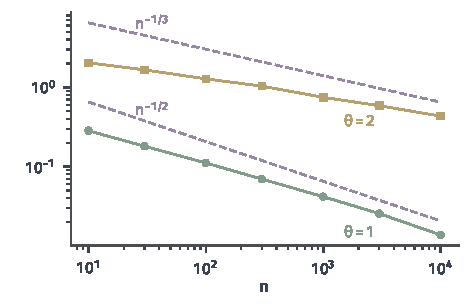
\includegraphics[width=80mm]{figures/07-probability/08-sampling-and-integration/matplotlib/pgrad-pareto-error/figure.pdf}
  \caption{同一例子中，$n$个导数样本平均的误差绝对值的中位数（每个$n$重复$2000$次，固定种子），双对数坐标。绿色圆点为$\theta=1$，黄色方块为$\theta=2$；紫色虚线是斜率为$-1/2$与$-1/3$的参考线。}
  \label{fig:pgrad-pareto-error}
\end{BookInlineFigure}

这个例子的教训适用于本章所有梯度估计：先用局部控制确认梯度可以写成期望，再单独检查梯度样本的二阶矩，二者不能互相代替。参数离可积性边界越近，导数样本的尾部越重，即使期望仍然有限，样本估计也会变得不可靠。
